\documentclass[11pt, oneside]{article}   	% use "amsart" instead of "article" for AMSLaTeX format


\usepackage[letterpaper, top=10mm, left=22mm, right=22mm]{geometry}
             		% See geometry.pdf to learn the layout options. There are lots.
              		% ... or a4paper or a5paper or ... 
%\geometry{landscape}                		% Activate for rotated page geometry
%\usepackage[parfill]{parskip}    		% Activate to begin paragraphs with an empty line rather than an indent
\usepackage{graphicx}				% Use pdf, png, jpg, or eps§ with pdflatex; use eps in DVI mode
								% TeX will automatically convert eps --> pdf in pdflatex
\usepackage{amssymb,amsmath,multirow,subfigure,comment}
  
\title{\bf HPC-Homework 5: Image convolution with OpenCL}
\author{\bf \large Ya Zhu}
\date{}							% Activate to display a given date or no date
\begin{document}
\maketitle 
\section{}
\begin{figure}[ht]\label{fig:1}
\centering
\subfigure[original photo]{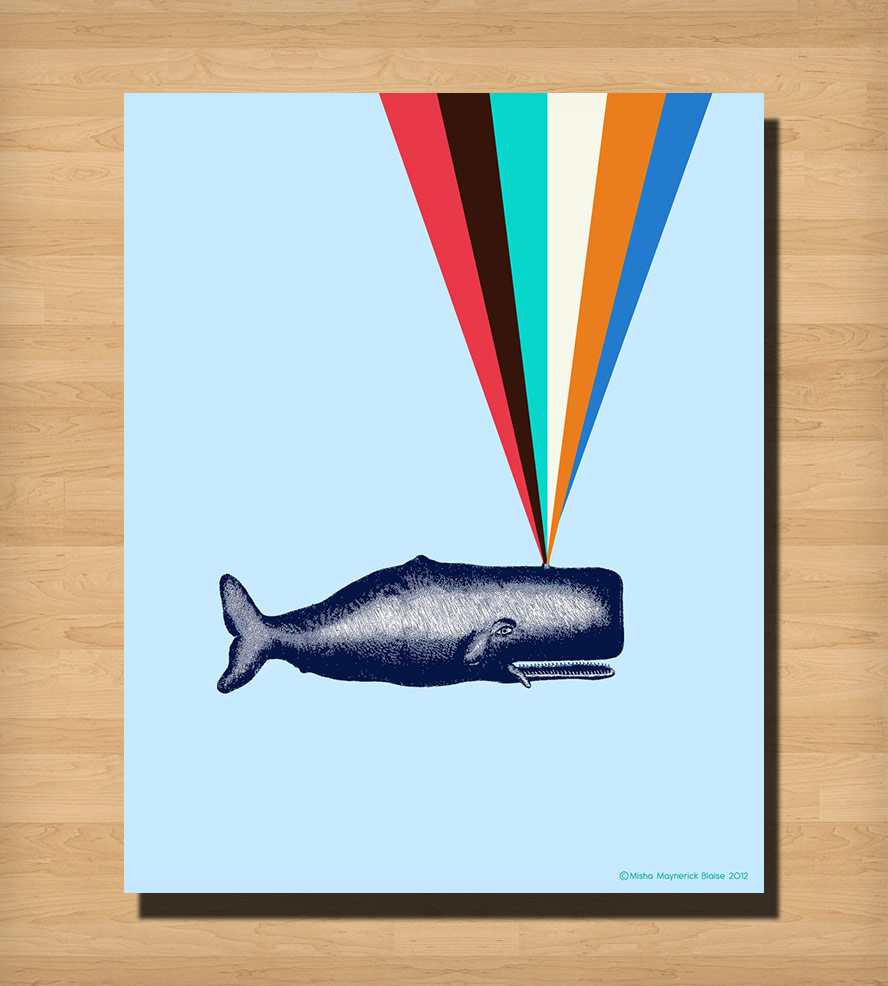
\includegraphics[width=0.45\linewidth]{fig/whale.png}}
\subfigure[blurred 100 times]{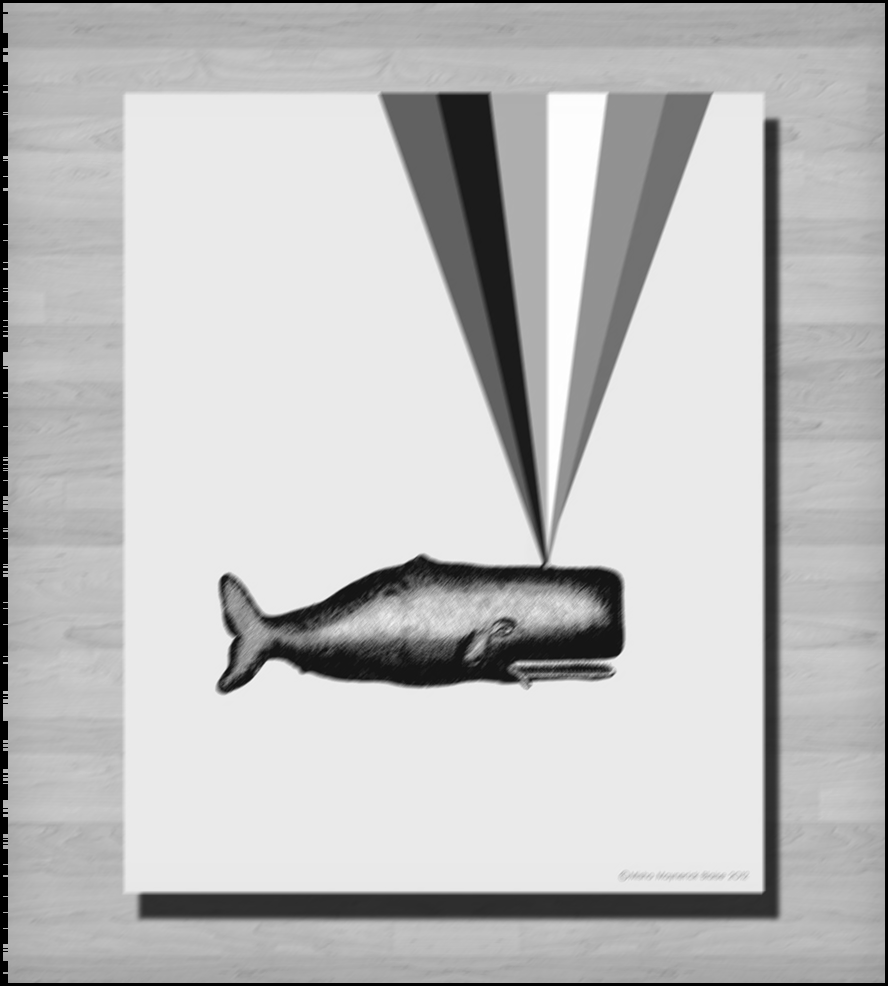
\includegraphics[width=0.45\linewidth]{fig/whale1.png}}
\caption{Result of blurring the same image at each iteration.}
\end{figure}
\begin{table}[h]
\centering
\caption{Statistics of different devices with different work group sizes.}
\label{tbl:1}
\begin{tabular}{|c|c|c|c|c|c|c|}
\hline
       & \multicolumn{3}{c|}{16, 16} & \multicolumn{3}{c|}{8, 8} \\ \hline
Device &    MPixels/s     &   GBit/s      &   GFlop/s      &    MPixels/s     &  GBit/s      &   GFlop/s     \\ \hline
MacPro &    317.188093     &    2.537505     &    15.442580     &    278.375138     &    2.227001    &  13.552937      \\ \hline
cuda3  &    212.853350     &   1.702827      &   10.362952      &  189.331240       &   1.514650     &   9.217757     \\ \hline
\end{tabular}
\end{table}
\section{}
\begin{figure}[ht]\label{fig:1}
\centering
\subfigure[original photo]{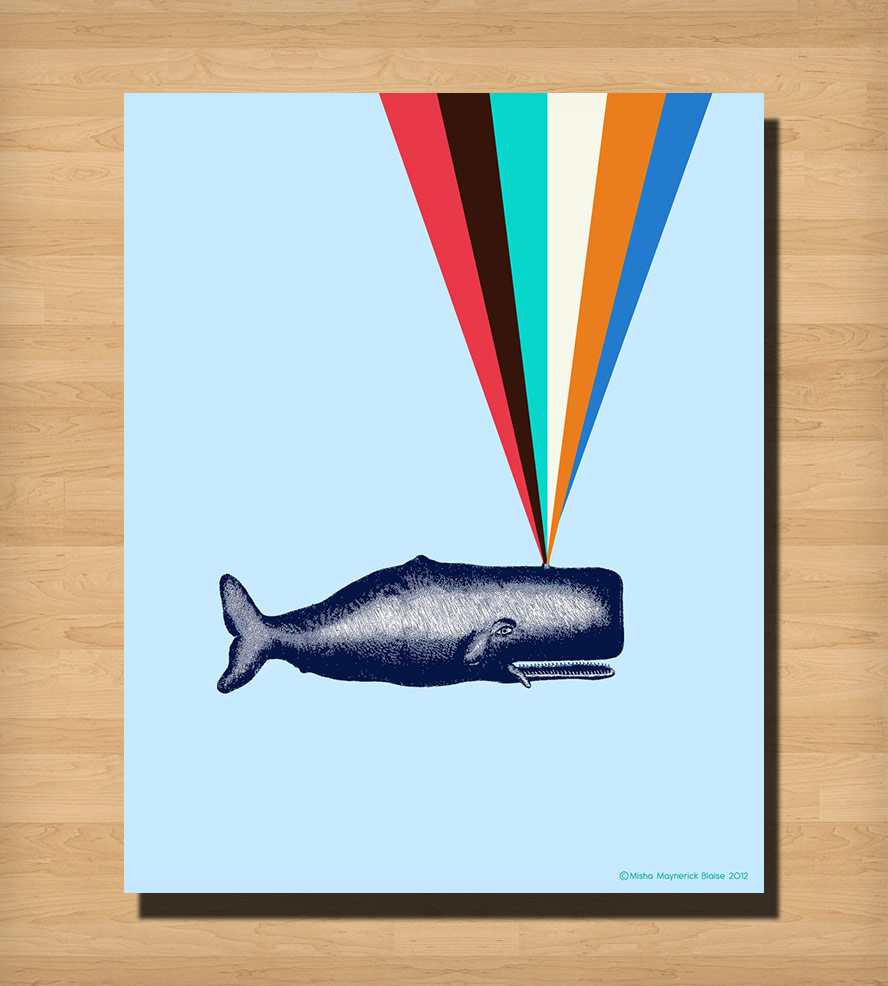
\includegraphics[width=0.45\linewidth]{fig/whale.png}}
\subfigure[blurred 100 times]{
\includegraphics[width=0.45\linewidth]{fig/whale2.png}}
\subfigure[blurred 1000 times]{
\includegraphics[width=0.45\linewidth]{fig/whale3.png}}
\subfigure[blurred 10000 times]{
\includegraphics[width=0.45\linewidth]{fig/whale4.png}}
\caption{Result of blurring the $k-1$th output image at $k$th iteration.}
\end{figure}
\end{document}  
